\section{Evaluation (3.5p)}

\subsection{Experiments (1p)}
\todo[inline]{Reduce the content}
\subsubsection{Experiment 1 - Breast Cancer Classification}

\begin{figure}[h]
    \centering
    \includegraphics[width=0.95\linewidth]{slides/scenario.png}
    \caption{Flow of classification and trust evaluation in PaTAS: From raw data to inference and trust assessment.}
    \label{fig:ptas-breast-cancer-flow}
\end{figure}

\paragraph{Overview}
\cref{fig:ptas-breast-cancer-flow} illustrates the complete flow of the system from dataset preparation to trust assessment. The process begins with the acquisition of ultrasound images, which are labeled and preprocessed for feature extraction. These features are used to train a neural network model for binary tumor classification (benign vs. malignant). During inference, query images undergo the same feature extraction pipeline and are classified by the trained model. In parallel, the PaTAS system evaluates the trustworthiness of the prediction by considering both the inference path and the trust associated with input features. The IPTA module computes a final trust score for the prediction.

\paragraph{Dataset}
We utilize the \href{https://archive.ics.uci.edu/dataset/17/breast+cancer+wisconsin+diagnostic}{Breast Cancer Wisconsin (Diagnostic) Dataset} from the UCI Machine Learning Repository, which comprises 569 samples. Each sample contains 30 numeric features derived from digitized images of fine needle aspirates (FNA) of breast masses. These features capture characteristics such as radius, texture, perimeter, area, smoothness, compactness, concavity, symmetry, and fractal dimension. Each of these characteristics is measured using three statistics: the mean, the standard error, and the worst (maximum) value. The objective of the neural network is to perform binary classification, distinguishing between benign and malignant tumors.

\paragraph{Neural Network Configuration}
The neural network employed in this experiment follows a simple architecture composed of an input layer with 30 neurons, a hidden layer with 16 neurons, and an output layer with 2 neurons, denoted as a 30-16-2 configuration. The ReLU activation function is applied in the hidden layer, while the Softmax function is used in the output layer. The model is trained over 5 epochs using a batch size of 64 and a learning rate of 0.2. Upon evaluation, the network achieves a test accuracy of 98\%, demonstrating strong performance on the classification task.

% \paragraph{PaTAS Configuration}
% The Parallel Trust Assessment System (PaTAS) is designed to mirror the structure of the neural network, thus also following a 30-16-2 layout. During inference, multiplication operations in the feedforward phase are handled using Subjective Logic (SL) trust discounting, while additions are processed via a generalization version of SL averaging fusion. The ReLU and Softmax activations are treated as identity mappings within PaTAS to preserve trust propagation semantics. At initialization, all weight parameters $\omega_\theta$ in the trust system are set to vacuous SL opinions, represented as $(0, 0, 1)$, indicating a complete lack of prior evidence about their trustworthiness.

\paragraph{Data Trust Assessment Functions}
To assess the sensitivity of the PaTAS under varying levels of trust in the input data, we defined three distinct trust profiles. These profiles are combined based on whether we are evaluating the label or the input features, resulting in a total of nine combinations. In the first profile, all inputs are treated as fully trusted, with trust opinions set to $(1,0,0)$ . In the second one, the data is considered fully distrusted, represented by the opinion $(0,1,0)$. Lastly, we consider a case where all inputs are fully uncertain, which is captured by the opinion $(0,0,1)$.

\paragraph{Causes of Input Untrustworthiness}
We simulate trust degradation in inputs to reflect realistic scenarios that could affect data reliability. For example, poor-quality imaging caused by faulty sensors may lead to corrupted or noisy features. Human errors in annotation can result in mislabeled instances, introducing incorrect supervision into the learning process. Additionally, flaws in the preprocessing pipeline (such as incorrect feature normalization or segmentation) can yield inaccurate numerical descriptors, further reducing trust in the data sample.

\subsubsection{Experiment 2 - MNIST Dataset}

\paragraph{Overview}
In this experiment, we evaluate the PaTAS framework on the MNIST dataset, a popular benchmark for handwritten digit classification. The flow of the system begins with the acquisition of the MNIST images, which are preprocessed and labeled. These grayscale images, each with dimensions 28x28 pixels, are used as input directly into the neural network model, which classifies the images into one of the 10 digits. During inference, query images undergo the same preprocessing, and the network performs classification. In parallel, the PaTAS framework evaluates the trustworthiness of the classification, and the IPTA module computes the final trust score based on the inference path and the pixel values.

\paragraph{Dataset}
For this experiment, we use the \href{http://yann.lecun.com/exdb/mnist/}{MNIST dataset}, a widely used benchmark for handwritten digit classification. The dataset consists of 60,000 training images and 10,000 test images, each representing one of the digits from 0 to 9. Each image is 28x28 pixels in grayscale, resulting in 784 input features per image. The goal of the neural network is to classify these images into one of the 10 digit classes.

\paragraph{Neural Network Configuration}
We tested three different neural network architectures with varying numbers of hidden neurons:

\begin{itemize}
    \item \textbf{Architecture 1:} Input layer with 784 neurons (28x28 grayscale pixels), one hidden layer with 5 neurons, and an output layer with 10 neurons (784-5-10 configuration).
    \item \textbf{Architecture 2:} Input layer with 784 neurons, one hidden layer with 10 neurons, and an output layer with 10 neurons (784-10-10 configuration).
    \item \textbf{Architecture 3:} Input layer with 784 neurons, one hidden layer with 20 neurons, and an output layer with 10 neurons (784-20-10 configuration).
\end{itemize}

Each model uses the ReLU activation function for the hidden layer and the Softmax activation function for the output layer. The models are trained for 5 epochs with a batch size of 64 and a learning rate of 0.2. Test accuracies achieved ranged from 94\% to 98\% depending on the architecture used.

% \paragraph{PaTAS Configuration}
% The PaTAS configuration for Experiment 2 is the same as in Experiment 1, with the architecture mirroring the neural network and corresponding layers. All weight parameters $\omega_\theta$ in the PaTAS system are initialized to vacuous SL opinions, represented as $(0, 0, 1, a)$.

\paragraph{Data Trust Assessment Functions}
In Experiment 2, we evaluate two different data trust assessment functions:
\begin{itemize}
    \item The first function always returns a fully uncertain/vacuous opinion for all inputs, reflecting complete uncertainty about the data. This approach represents a scenario where the model has no prior trust in any of the inputs, treating all pixels equally as uncertain.
    \item The second function uses a randomized trust assessment, where each input is assigned a trust opinion based on a probabilistic method. Specifically, the trust assessment is based on a biased triplet (trust, distrust, vacuous), where:
    \begin{itemize}
        \item Every third input receives a trust opinion, indicating a belief in the input.
        \item Another third receives a distrust opinion, indicating skepticism.
        \item The remaining third receives a vacuous opinion, reflecting no prior trust knowledge or complete uncertainty.
    \end{itemize}
    This randomization introduces variability in the trust level for each input, simulating different levels of uncertainty across the dataset.
\end{itemize}

These two functions allow us to compare the impact of a constant uncertainty approach versus a more varied, randomized trust assignment on the PaTAS framework’s performance.


\paragraph{Causes of Data Untrustworthiness}
In this experiment, we hypothesize that the degradation of input trust can result from various factors that impact the quality of the MNIST dataset. These include noisy images caused by poor-quality digit scans, errors in the digit labels due to human annotation mistakes, and inaccuracies in preprocessing. Additionally, any distortion or incorrect scaling of pixel values during normalization may lead to a loss of trust in the image data.


\subsubsection{Experiment 3 - Poisoned MNIST Dataset}

\paragraph{Overview}
In this experiment, we evaluate the PaTAS framework on a poisoned version of the MNIST dataset. The objective is to test how well the system handles adversarial perturbations and poisoned data. The poisoned dataset is created by maliciously altering a subset of the training data. The neural network is then trained on this corrupted dataset, and the PaTAS framework is used to assess the trustworthiness of the predictions.

\paragraph{Dataset}
The poisoned dataset is based on the original \href{http://yann.lecun.com/exdb/mnist/}{MNIST dataset}, with modifications made by three parties:
\begin{itemize}
    \item Two parties provide clean, uncorrupted data.
    \item One malicious party introduces corruption by flipping the labels of a subset of images with digits 6 and 9. These label flips simulate intentional mislabeling in the dataset.
    \item Additionally, the malicious party adds a patch of a given size at the top-left corner of a portion of the images, further corrupting the training data.
\end{itemize}
This corrupted dataset simulates a data poisoning attack, where adversarial examples can degrade the model's performance and potentially mislead it during inference.

\paragraph{Neural Network Configuration}
We used \textbf{Architecture 3} of previous experiment. An input layer with 784 neurons, one hidden layer with 20 neurons, and an output layer with 10 neurons (784-20-10 configuration).

% \paragraph{PaTAS Configuration}
% The PaTAS configuration for Experiment 3 is the same as in Experiment 1 and Experiment 2.

\paragraph{Data Trust Assessment Functions}
For the poisoned dataset, we assign trust to the pixels and labels based on the corruption introduced by the malicious party. Specifically:
\begin{itemize}
    \item The pixels corresponding to the patch added by the malicious party are considered distrusted, while all other pixels are considered trusted.
    \item The labels corresponding to the digits 6 and 9 are considered distrusted, while the labels for other digits are considered trusted.
\end{itemize}
This allows the PaTAS framework to focus on the portions of the data that are likely to have been corrupted, while trusting the rest of the input.


\paragraph{Causes of Input Untrustworthiness}
In this experiment, the degradation of input trust is introduced through data poisoning. The poisoned MNIST dataset includes noisy images due to random pixel modifications and mislabeled instances that corrupt the training process. These corrupted samples introduce uncertainty and potential adversarial patterns that may negatively affect the performance and trustworthiness of the model during inference.

\subsection{Implementation}
\todo[inline]{Trust learning rate}

During inference, multiplication operations in the feedforward phase are handled using Subjective Logic (SL) trust discounting, which adjusts the weight of each connection based on the trust assigned to the inputs. For additions, we use a generalized version of SL averaging fusion, which is necessary to handle the summation of multiple values. This is essential because the addition operations inside the neural network involve more than two inputs (not just binary operations). Thus, the operator must either be generalized or, at a minimum, be associative and commutative, to ensure proper trust propagation across all neurons.

for trust feed forward we use (SL discounting for multiplication and SL averaging fusion for addition).
To handle trust revision, we use the same operator for \(\ominus, \bigwedge\,\text{and} \bigoplus \). 

We implemented the PaTAS framework and neural network models in Python. Two main modules were created: PrimaryNN and PaTAS. PrimaryNN handles the neural network structure, training, and inference operations and PaTAS implements all the functions and operations needed for trust assessment and propagation, as specified in PaTAS Operation (referenced in \ref{fig:ptasoperation}).
Both modules interact seamlessly to enable the PaTAS framework to evaluate and revise trust dynamically during each forward pass and backpropagation phase.

The full implementation of the PaTAS framework and the neural network models is available on GitHub. You can access the code repository on github~\cite{code}. This includes all the necessary modules, dependencies, and instructions for running the experiments as described in this paper.


\subsection{Results (2p)}
In this paper, the evaluation of the Parallel Trust Assessment System (PaTAS) is conducted during the training phase of the neural network. After each round of training (i.e., a complete feedforward and backpropagation cycle), we assess the trustworthiness of the input data using three distinct input types:

\begin{itemize}
    \item Fully Trusted Input: where the trust in the data is considered absolute (row 1 in each figure).
    \item Fully Uncertain Input: where the trust in the data is undefined, represented as maximum uncertainty (row 2 in each figure).
    \item Fully Distrusted Input: where the data is assumed to be unreliable, and the trust is considered to be fully negative (row 3 in each figure).
\end{itemize}

For each of these three input types, we track and plot the evolution of three key metrics over the course of training:

\begin{itemize}
    \item Trust Mass: representing the level of confidence in the given input.
    \item Uncertainty Mass: representing the uncertainty associated with the input's trustworthiness.
    \item Distrust Mass: representing the level of disbelief in the input.
\end{itemize}

As a result, for each evaluation, 9 distinct plots are generated, corresponding to the 3 input types (fully trusted, fully uncertain, and fully distrusted) and each of the three key metrics (trust, uncertainty, and distrust).

% \todo[inline]{NO IPTA? think of IPTA when data poisoned}

\subsubsection{Overall Results}
All the results are depicted in Figures~\ref{fig:cancer0.01}~\ref{fig:cancer0.1}\ref{fig:mnist}\ref{fig:mnistpois}\ref{fig:mnistrand}. The overall results of the evaluation provide confirmation of several key theoretical properties of PaTAS, which were proven in Section~\ref{sec:ptastheory}. Specifically, the evaluation supports the following findings:

\begin{itemize}
    \item \textit{Convergence of Trust Assessment:} The evaluation confirms that the trust assessment converges as expected, which aligns with the theoretical results proved.
    \item \textit{PaTAS Inference on Vacuous Input Yields Vacuous Output:} As proven in Section \ref{sec:theory}, when the input is vacuous (i.e., fully uncertain), the PaTAS inference also results in a vacuous output. This can be seen in all figure 
    \item \textit{Symmetric Inference under PaTAS:} The symmetry property of PaTAS, as discussed in Section~\ref{sec:ptassyminv}, is observed. This property ensures that the inference remains symmetric when the input trust assessments are symmetric.
\end{itemize}

These overall results serve as strong validation for the theoretical foundations of PaTAS and provide confidence in the robustness and reliability of the system.

For the detailed analysis, we will focus only on the 3 plots corresponding to the evolution when assessing a trustworthy input. This is because the results from processing uncertain inputs naturally lead to uncertain outputs, as expected. Additionally, there exists symmetry between the results when processing fully trusted and fully distrusted inputs. Therefore, we can deduce that a similar behavior will be observed when analyzing the distrusted input, without needing to analyze it in detail. Thus, the primary focus can remain on the evolution of trust, uncertainty, and distrust when the input is fully trusted.
Moreover, we notice that in most of the plots, when the input is fully trusted, the distrust mass in the output remains generally close to zero throughout the training rounds. This consistency suggests that the distrust component does not significantly contribute to the overall assessment when the input is highly reliable. Consequently, we decide to analyze only the trust mass (whenever the distrust mass does not present significant results), as the sum of uncertainty and trust remains approximately 1.







\subsubsection{Experiment 1 - Breast Cancer Classification~\ref{fig:cancer0.01}~\ref{fig:cancer0.1}}

We conducted the experiment for two values of \(\epsilon\) (0.1 and 0.01) to observe how the system behaves under different levels of threshold for the \(\delta\) values.

The behavior remains largely consistent, particularly when the features dataset \(X\) is distrusted. Regardless of the trust of the labels dataset \(Y\) and the \(\epsilon\) value, the results are the same. At the beginning of the training, the trust mass is around 0.25. After just one training round, the trust mass drops to zero.

\paragraph{For \(\epsilon = 0.01\)} 
When \(X\) is fully uncertain, we observe similar trends regardless of whether \(Y\) is distrusted, vacuous, or trusted. When \(Y\) is distrusted, initially, the trust mass is around 0.23. After just a few rounds, the trust mass increases slightly to 0.28. After around two epochs, the trust mass dips to 0.20 before gradually rising and stabilizing at around 0.28. 
The behavior is almost identical when \(Y\) is vacuous, except for the bottom peak of trust mass (around 0.14 instead of 0.23) and the top peak of uncertainty mass (around 0.86 instead of 0.77).
When \(Y\) is fully trusted, the behavior is nearly the same, but the final values are slightly better. The trust mass stabilizes at 0.30 (compared to 0.28), and the uncertainty mass reaches 0.70 (better than 0.72).

When \(X\) is fully trusted, we observe the following evolution: initially, the trust mass starts at 0.2, then rises sharply to 0.8, 0.7, or 0.6 depending on whether \(Y\) is distrusted, fully uncertain, or trusted, respectively. After this rapid increase, the trust mass drops slightly before gradually rising again and stabilizing at 0.8.

\paragraph{For \(\epsilon = 0.1\)}
With a larger value of \(\epsilon\), the creation process becomes less sensitive to the \(\delta\) values. Specifically, when \(\epsilon\) is too large, almost all the \(\delta\) values lead to similar quantified values of \(T_{\theta_i \mid y_{\text{batch}}}\) (cf. the algorithm). This effect is particularly noticeable at the beginning of the training process, where the \(\delta\) values are typically large and contribute less variability to the trust calculations.

In the case where \(X\) is fully uncertain, the trust mass converges to 0.28 when \(Y\) is distrusted, to 0.30 when \(Y\) is fully uncertain, and to 0.34 when \(Y\) is fully trusted.

For fully trusted \(X\), the trust mass behaves as follows: when \(Y\) is distrusted, it stabilizes at 0.8; when \(Y\) is fully uncertain, it reaches 0.83; and when \(Y\) is fully trusted, it stabilizes at 0.9.

\paragraph{Key Observations} 
The trust in \(X\) has a more impact on the final results. As the trust in \(X\) increases, the influence of \(Y\)'s trust on the final output becomes more pronounced. The final trust values are higher when \(X\) is fully trusted, and the model appears to perform better when \(X\) is reliable.

These findings highlight the importance of the input trustworthiness in shaping the final results, confirming the sensitivity of the PaTAS to the data’s trust properties.

Another key remark is that when \(\epsilon\) is too small, whether \(Y\) is trusted, uncertain or distrusted does not really impact the final trust mass after convergence.
\todo[inline]{to discuss in the discussion}


\begin{table}[ht]
\centering
\begin{tabular}{|c|c|c|}
\hline
Trust Assessment & For \(\epsilon = 0.01\) & For \(\epsilon = 0.1\) \\
\hline
\(X\) fully uncertain, \(Y\) distrusted & 0.28 & 0.28 \\
\hline
\(X\) fully uncertain, \(Y\) vacuous & 0.28 & 0.30 \\
\hline
\(X\) fully uncertain, \(Y\) fully trusted & 0.30 & 0.34 \\
\hline
\(X\) fully trusted, \(Y\) distrusted & 0.8 & 0.8 \\
\hline
\(X\) fully trusted, \(Y\) fully uncertain & 0.79 & 0.83 \\
\hline
\(X\) fully trusted, \(Y\) fully trusted & 0.79 & 0.9 \\
\hline
\end{tabular}
\caption{Summary of final trust mass for the Breast Cancer Classification Experiment.}
\label{tab:cancer_results}
\end{table}


\subsubsection{Experiment 2 - MNIST Dataset}

\paragraph{Key Observations}
As shown by results of experiment 2, the bigger architecture the more trustworthy because smaller \( \delta \). Due to a lack of resources we couldn't evaluate our framework with bigger neural network



\subsubsection{Experiment 3 - Poisoned MNIST Dataset}


\todo[inline]{What does IPTA shows}
















% \begin{table}[htbp]
% \centering
% \scriptsize
% \renewcommand{\arraystretch}{1.3}
% \setlength{\tabcolsep}{4pt}

% \begin{tabularx}{\textwidth}{|c|c|c|c|}
% \hline

% & \textbf{Fully Trusted Data Trust Assessment Function} 
% & \textbf{Fully Un-Trusted Data Trust Assessment Function} 
% & \textbf{Fully Dis-Trusted Data Trust Assessment Function} \\
% \hline

% \textbf{Operation on the first data of the test dataset} & 
% Belief: 0.856 \newline Disbelief: 0.042 \newline Uncertainty: 0.102 & 
% Belief: 0.287 \newline Disbelief: 0.05 \newline Uncertainty: 0.663 & 
% Belief: 0.0 \newline Disbelief: 1.0 \newline Uncertainty: 0 \\
% \hline

% \textbf{Feed Forward + Aggregation on Tx fully trust opinion} & 
% Belief: 0.846 \newline Disbelief: 0.053 \newline Uncertainty: 0.102 & 
% Belief: 0.298 \newline Disbelief: 0.043 \newline Uncertainty: 0.659 & 
% Belief: 0.0 \newline Disbelief: 1.0 \newline Uncertainty: 0 \\
% \hline

% \textbf{Feed Forward + Aggregation on Tx fully un-trust opinion} & 
% Belief: 0.839 \newline Disbelief: 0.053 \newline Uncertainty: 0.108 & 
% Belief: 0.296 \newline Disbelief: 0.043 \newline Uncertainty: 0.661 & 
% Belief: 0.0 \newline Disbelief: 1.0 \newline Uncertainty: 0 \\
% \hline

% \textbf{Feed Forward + Aggregation on Tx fully dis-trust opinion} & 
% Belief: 0.0 \newline Disbelief: 1.0 \newline Uncertainty: 0 & 
% Belief: 0.0 \newline Disbelief: 1.0 \newline Uncertainty: 0 & 
% Belief: 0.0 \newline Disbelief: 1.0 \newline Uncertainty: 0 \\
% \hline
% \end{tabularx}

% \caption{Comparison of PaTAS trust outputs under different Data Trust Assessment Functions}
% \label{tab:ptas_subjective_logic}
% \end{table}

% \begin{figure}
%     \centering
%     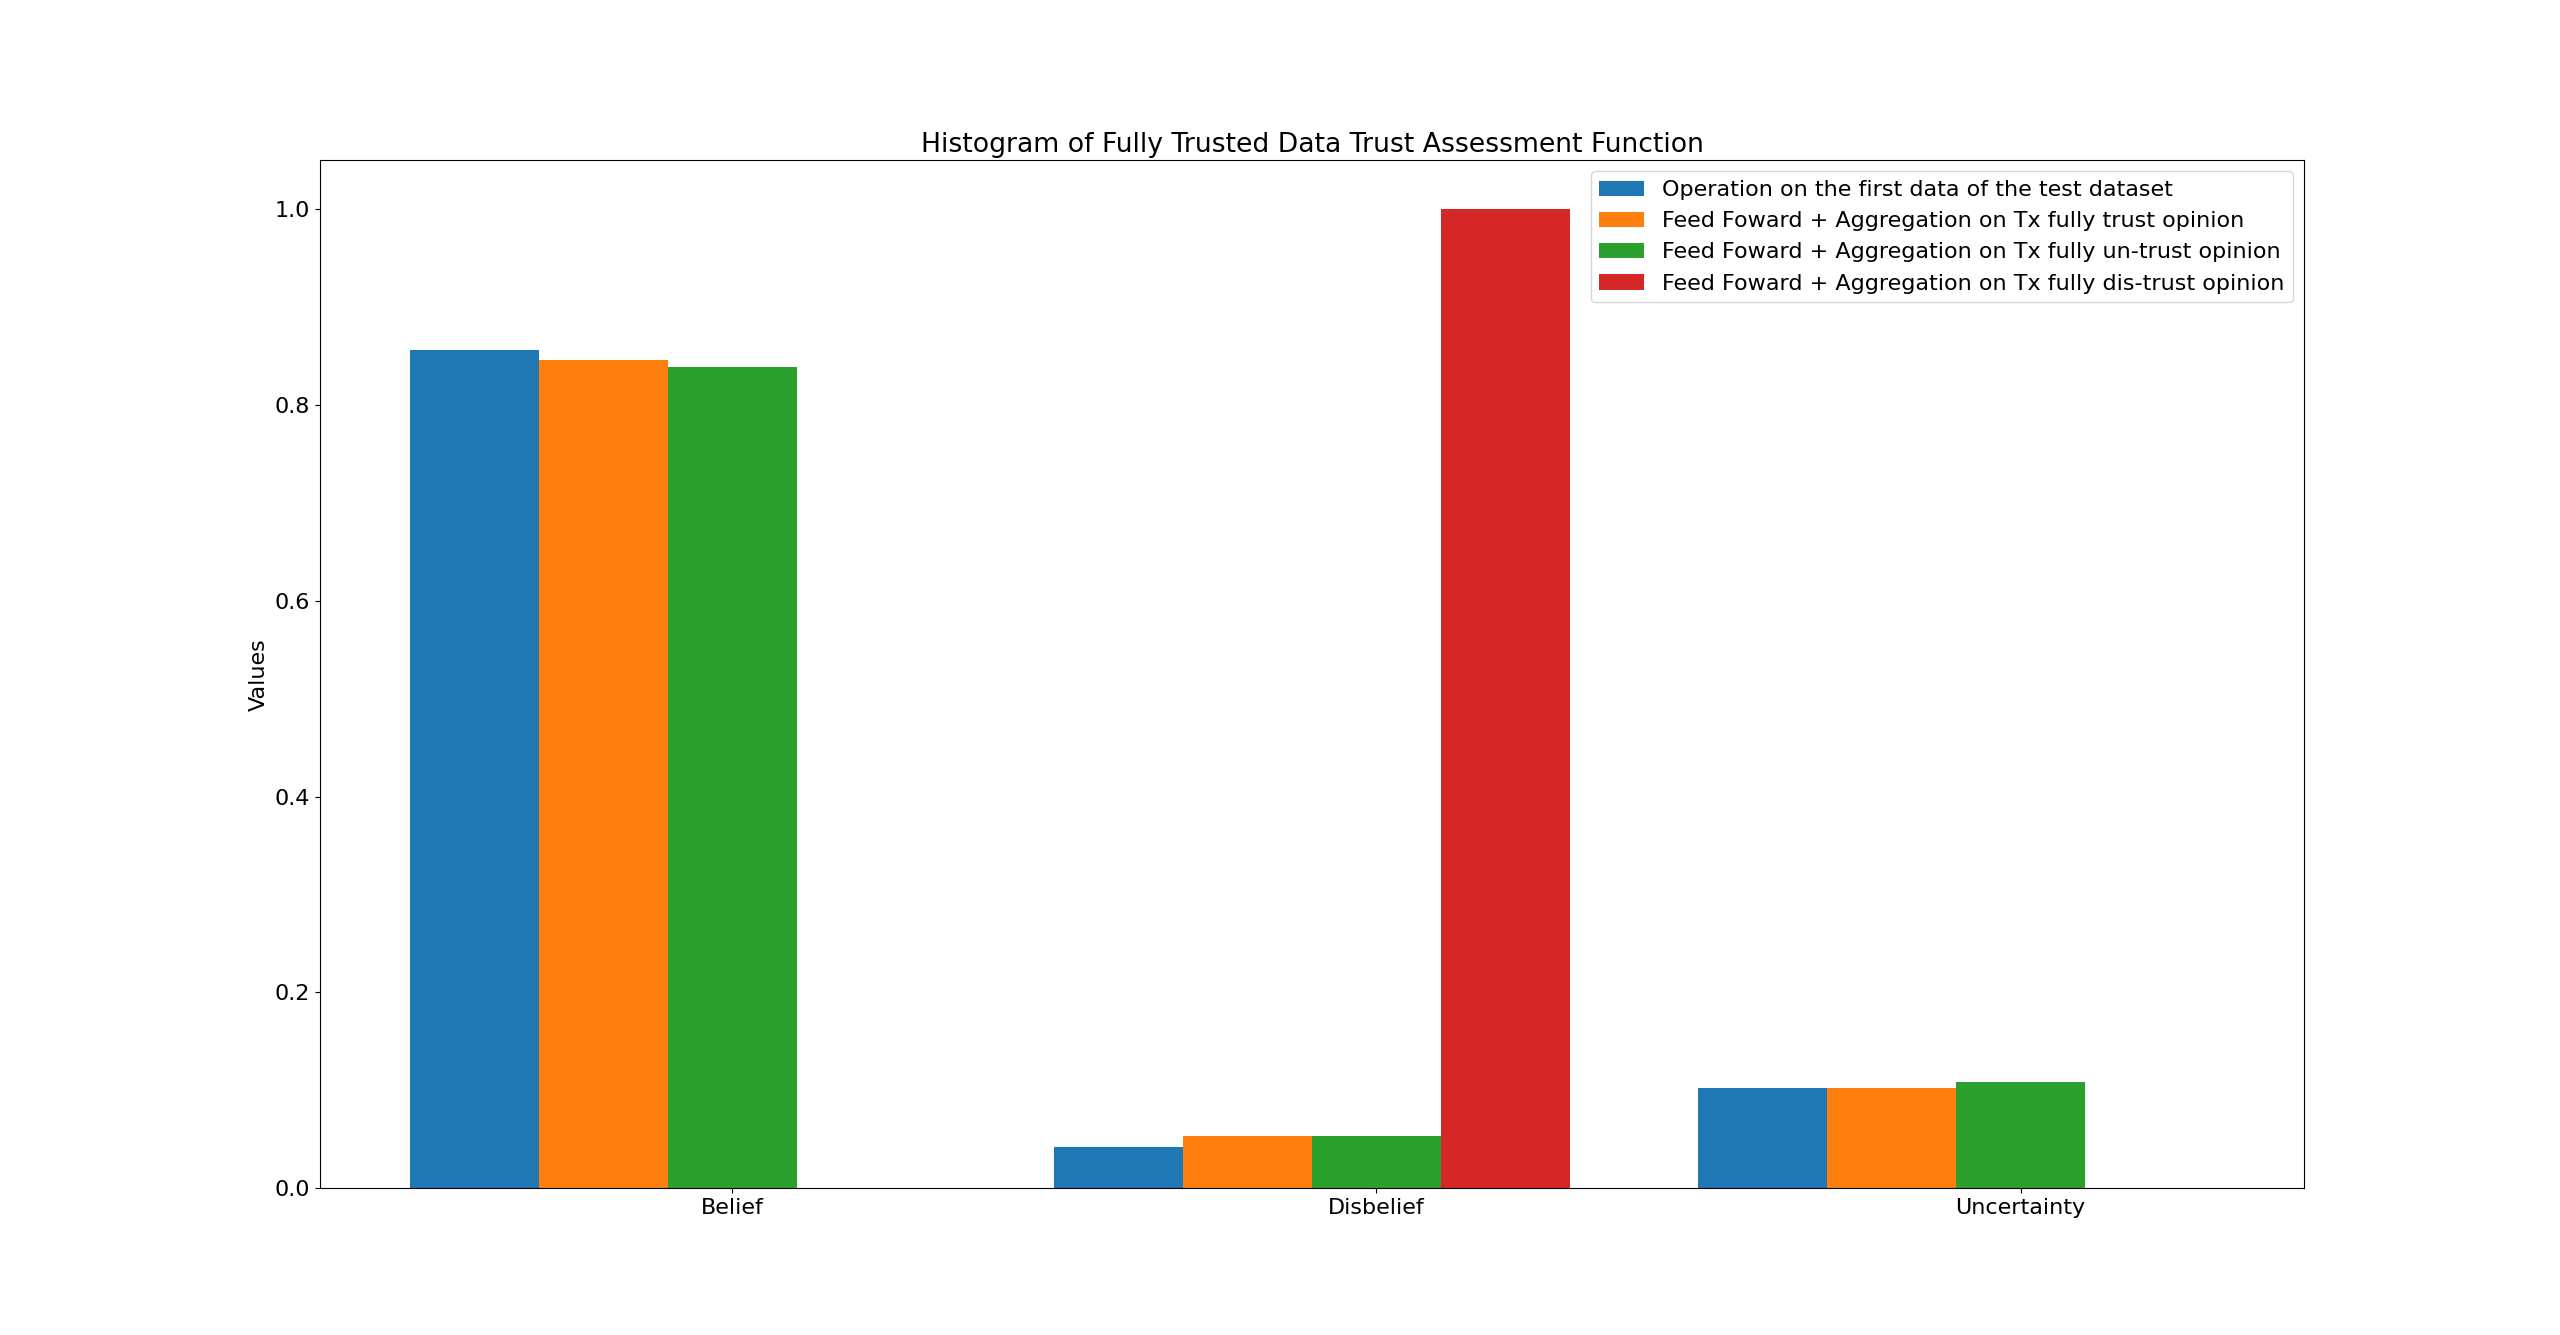
\includegraphics[width=0.5\linewidth]{sections/Ttrust.png}
%     \caption{Trust}
%     \label{fig:ttrust}
% \end{figure}
% \begin{figure}
%     \centering
%     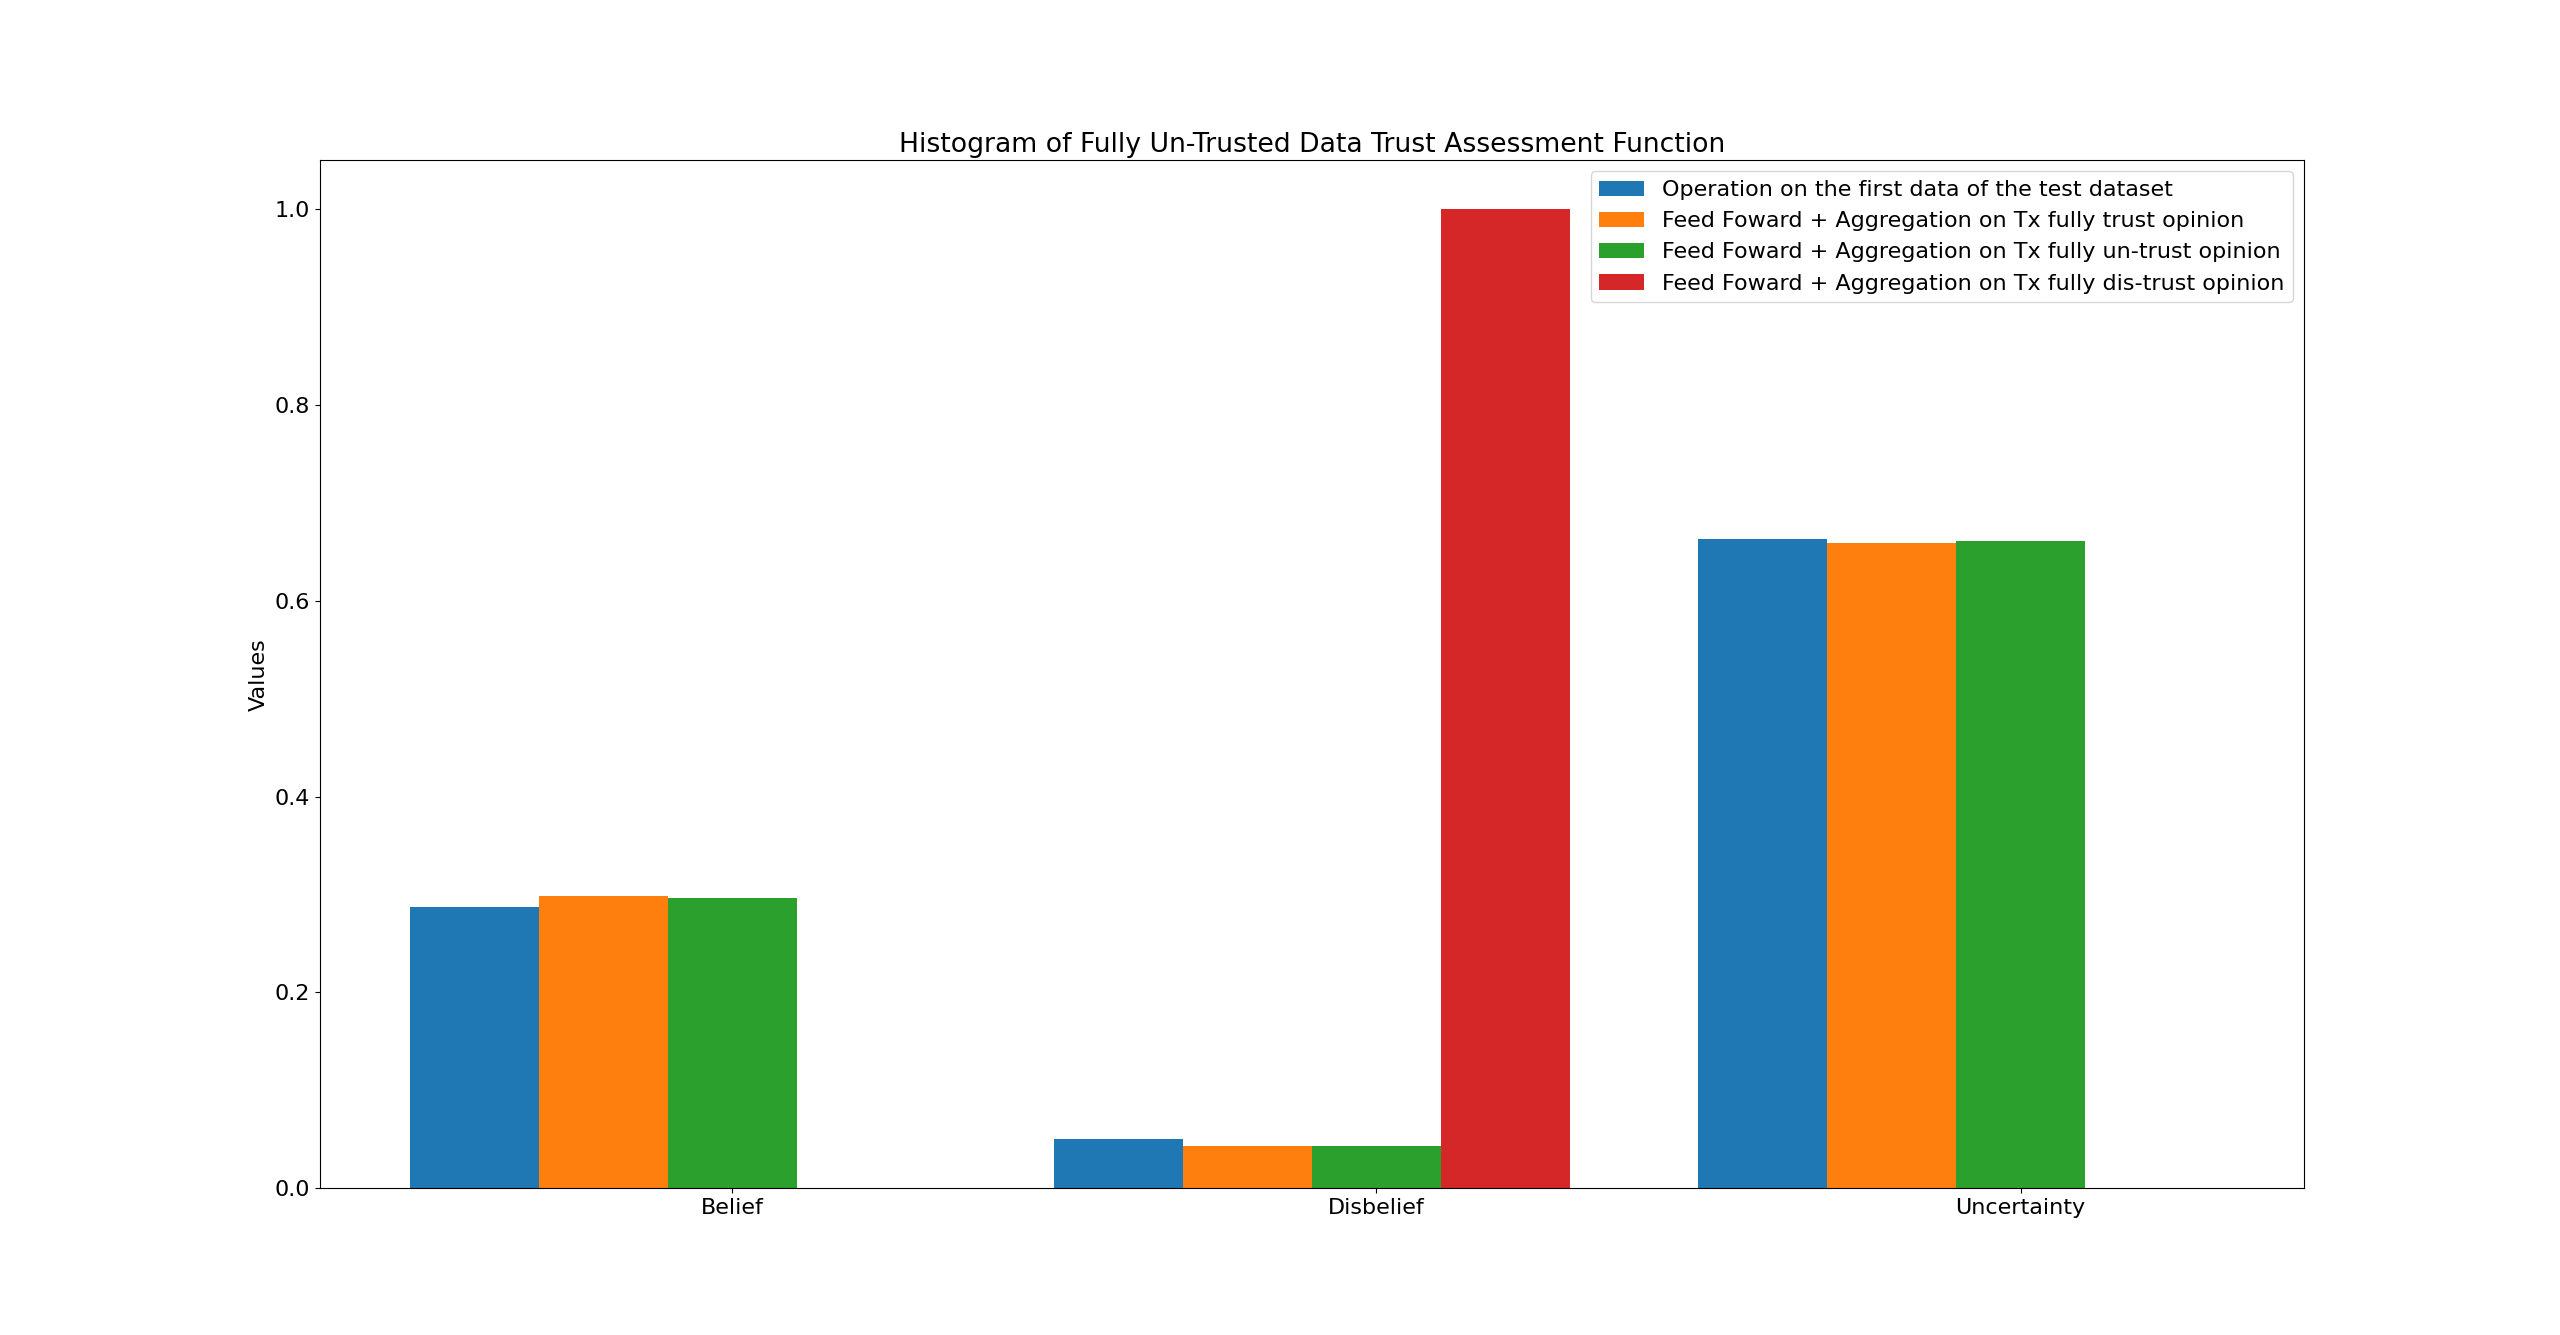
\includegraphics[width=0.5\linewidth]{sections/Tvacuous.png}
%     \caption{Untrust}
%     \label{fig:tutrust}
% \end{figure}
% \begin{figure}
%     \centering
%     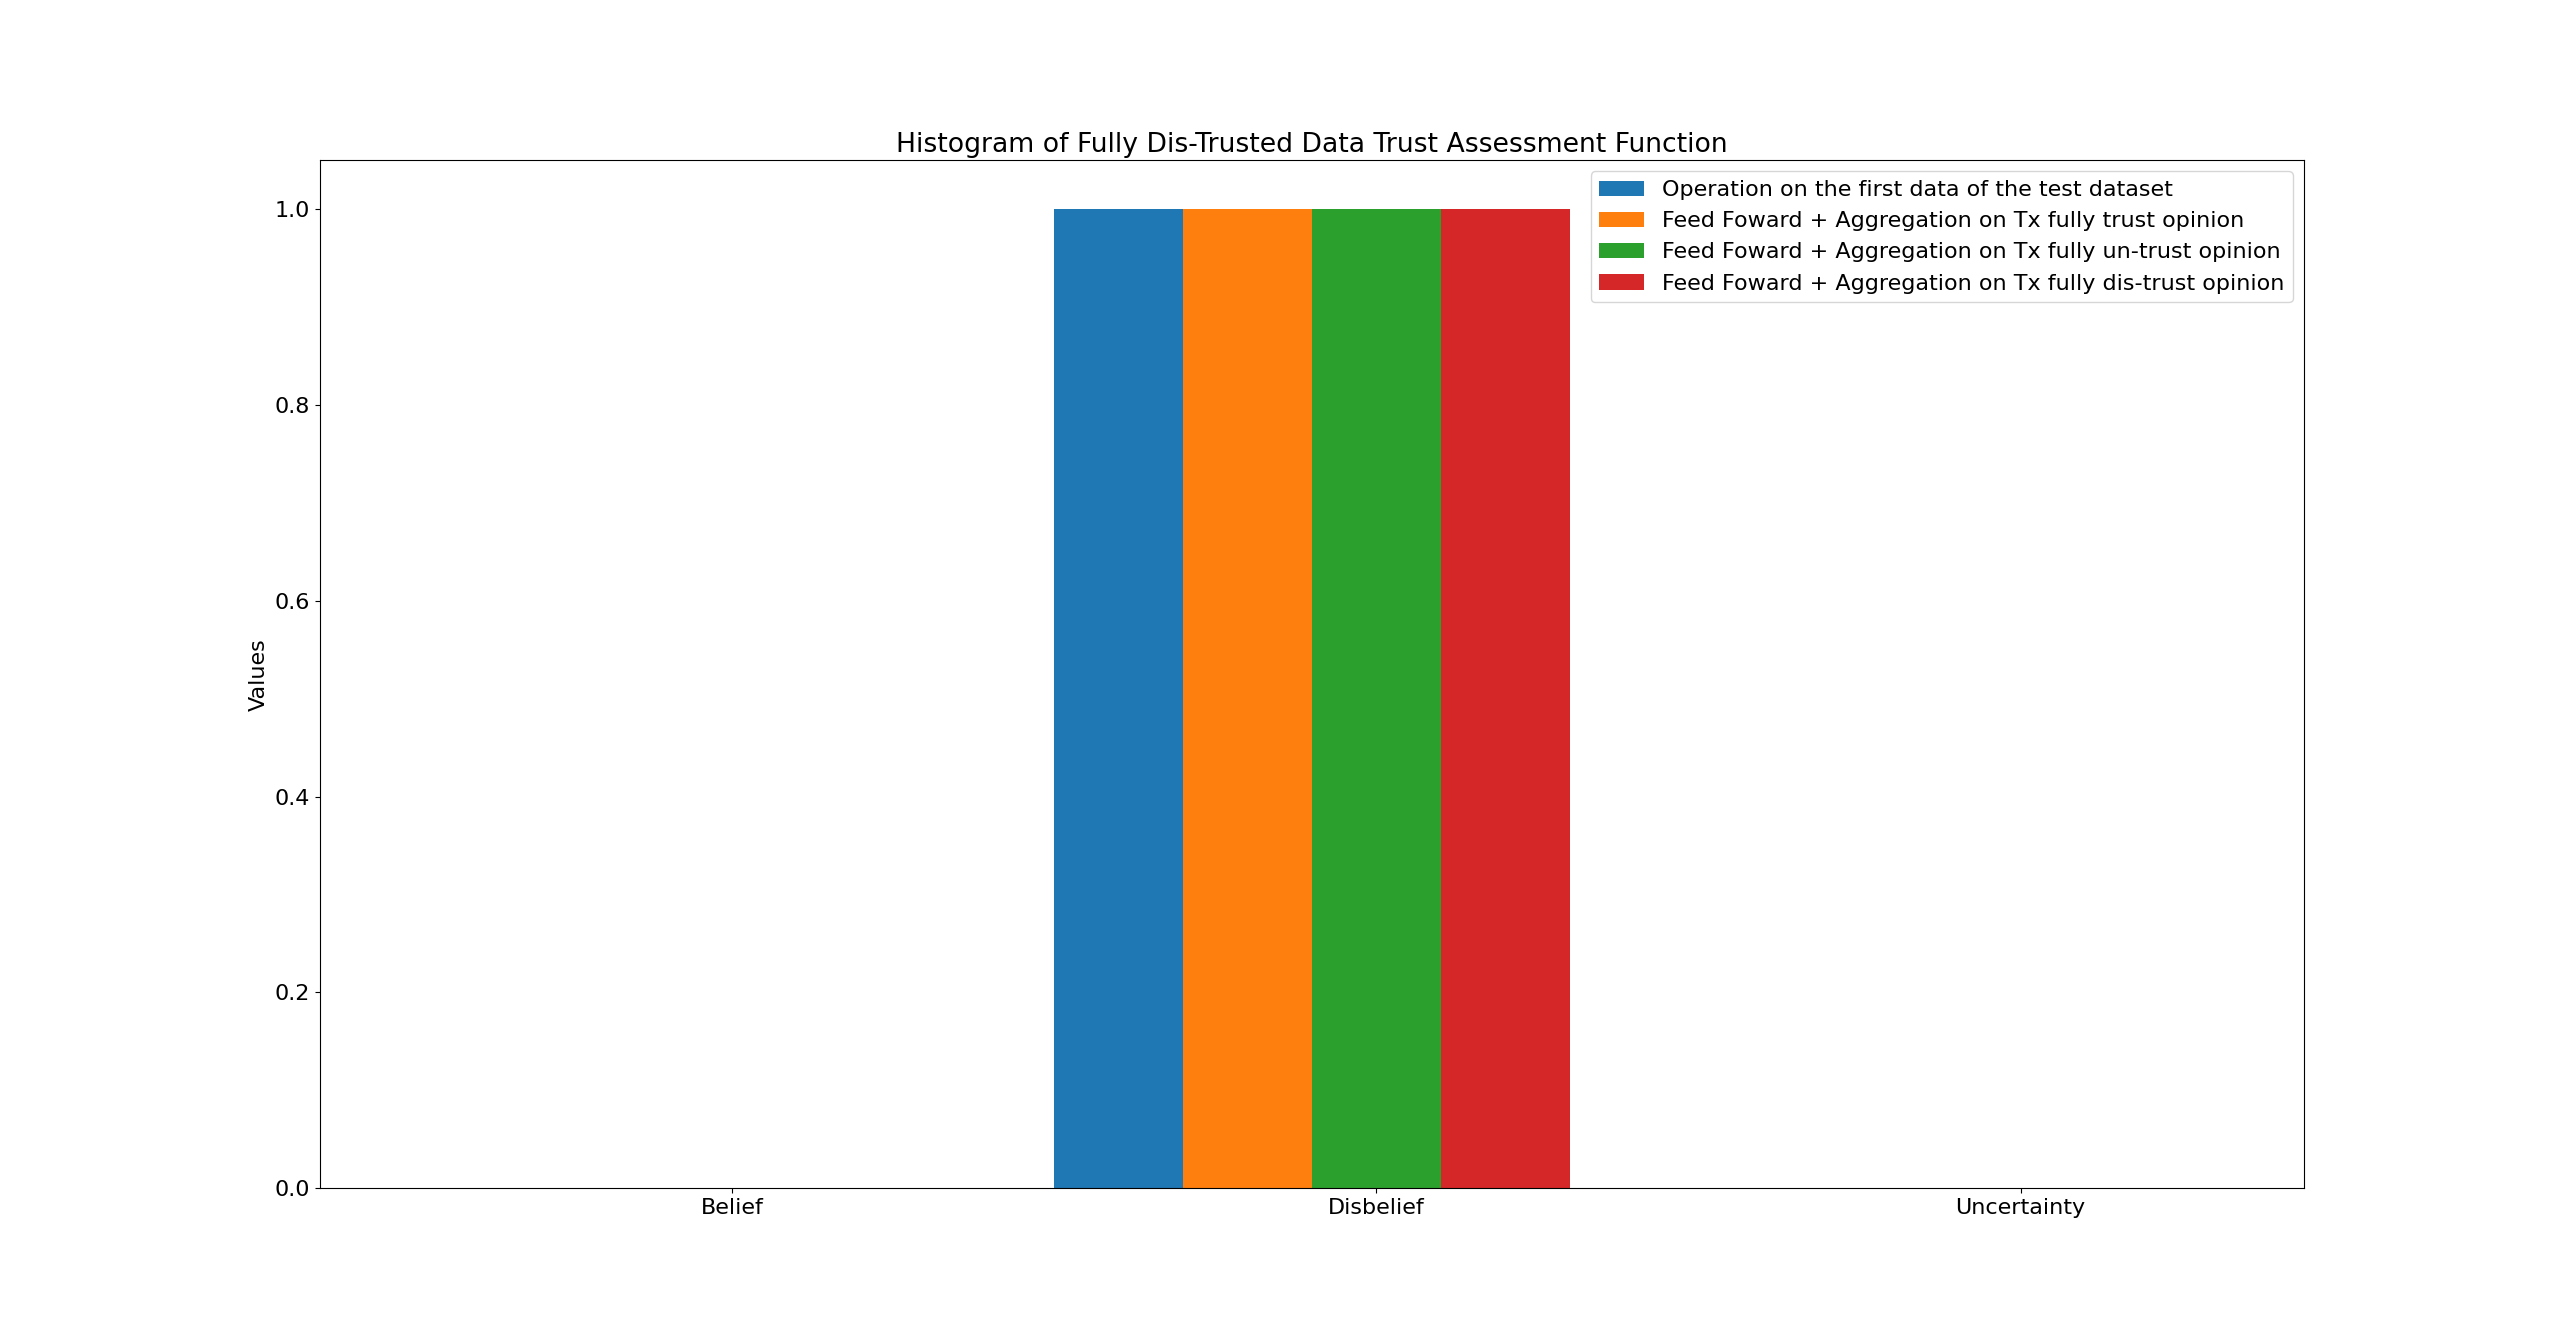
\includegraphics[width=0.5\linewidth]{sections/Tdistrust.png}
%     \caption{DisTrust}
%     \label{fig:tdtrust}
% \end{figure}



% Explain quickly what is Data poisonning attack: 
% https://ieeexplore.ieee.org/stamp/stamp.jsp?tp=&arnumber=8685687

% Create two parallel function:
% -one when the data is poisoned. create easily the dataset {data untrustworthy: (0.1, 0.8, 0.1) ; data trustworthy: (0.8,0.1,0.1)}
% -one when data is not poisoned and compare


% \subsection{ParaFunc result}
% Architecture, batch order...

% $\theta$ always same opinion $=>$ makes sense since same evidence and same initialization. 